%\begin{tcolorbox}
%Teilt eure Klassendiagramme bitte auf und baut \textbf{kein} einzelnes riesiges Diagramm.
%Getter und Setter Methoden müssen hier nicht modelliert werden.
%Sie sollten aber der klassischen Namenskonvention folgen, um die Nutzung in Sequenzdiagrammen zu ermöglichen.
%\\\\
%Auf jedes Diagramm folgt eine Tabelle, in der die Aufgabe \textbf{jeder} Klasse beschrieben wird.
%\end{tcolorbox}

\section{Frontend}

\subsection{Web}

\begin{figure}[h]
	\centering
	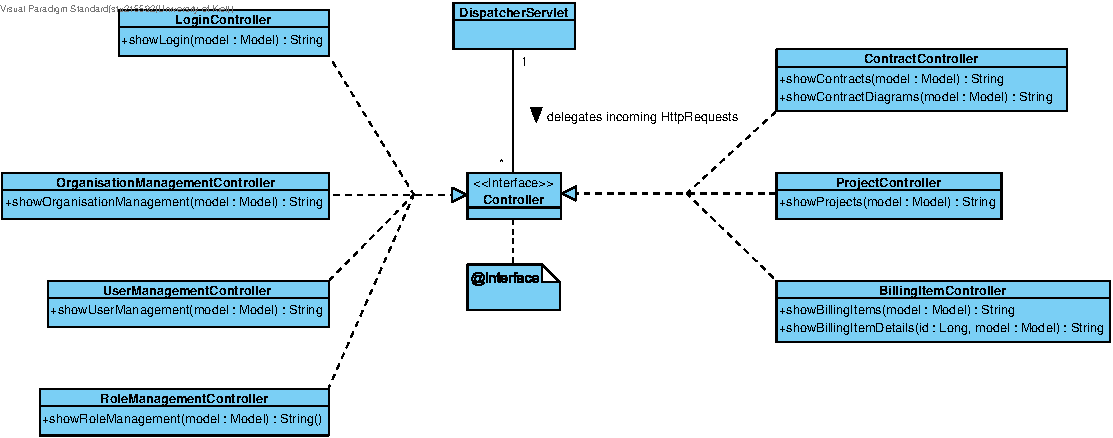
\includegraphics[width=\linewidth]{img/diagrams/Frontend Classes.pdf}
	\caption{Klassendiagramm - Frontend Web}
	\label{fig:klassendiagramm-web}
\end{figure}

\noindent
Klassen, deren Name mit ''Controller'' aufhört, verarbeiten HTTP Requests zu bestimmten Pfaden.
Die zu verarbeitenden Pfade sind pro Gebiet in einem jeweiligen Controller gruppiert.
In der folgenden Tabelle werden für Controller unter ''Aufgabe'' die zu verarbeitenden Pfade sowie deren Bedeutung aufgeführt.

\begin{table}[h]
	\centering
	\begin{tabularx}{\textwidth}{X X}
		\rowcolor[HTML]{C0C0C0} 
		\textbf{Klassenname} & \textbf{Aufgabe} \\
		DispatcherServlet & Leitet die HTTP Requests an den jeweils zuständigen Controller weiter \\
		\rowcolor[HTML]{E7E7E7} 
		LoginController & /login $\rightarrow$ Login-Seite \\
		OrganisationManagementController & /organisation_management $\rightarrow$ Seite für das Management von Organisationen und deren OrgAdmins \\
		\rowcolor[HTML]{E7E7E7} 
		UserManagementController & /user_management $\rightarrow$ Seite für das Management von WebUsern \\
		RoleManagementController & /role_management $\rightarrow$ Seite für das Management von Rollen \\
		\rowcolor[HTML]{E7E7E7} 
		ContractController & /contracts $\rightarrow$ Diese Seite zeigt Verträge an, für welche der WebUser die nötigen Berechtigungen hat \newline
		/contract_diagrams $\rightarrow$ Diese Seite zeigt Diagramme zu Verträgen an, für welche der WebUser die nötigen Berechtigungen hat \\
		ProjectController & /projects $\rightarrow$ Diese Seite zeigt Projekte an, für welche der WebUser die nötigen Berechtigungen hat \\
		\rowcolor[HTML]{E7E7E7} 
		BillingItemController & /billing_items $\rightarrow$ Diese Seite zeigt Leistungspositionen an, für welche der WebUser die nötigen Berechtigungen hat \newline
		/billing_item/\{ID\}/details $\rightarrow$ Diese Seite zeigt Details zu einer Leistungsposition mit gewählter ID an
	\end{tabularx}
	\caption{Klassenbeschreibung - Frontend Web}
	\label{table:klassenbeschreibung-web}
\end{table}

\clearpage

\subsection{App}

\section{Backend}
